\section{Classification Methods}
\label{sec:Approach}

In this chapter, we explain the method of classifying Twitter users
based on the target specificity of their information publishing defined
in \ref{sec:Target Specificity}.  In addition, in regards to Twitter
users classified into ``the target specificity is high'' by the above
method, we explain the method of determining why their target
specificities are high based on the result of our analysis mentioned in
\ref{subsec:The Causes}.

Figure~\ref{fig:Flow} shows the overall flow of our methods.  First, we
apply the method explained in \ref{subsec:Classification Step1} to
Twitter users and classify them into two categories: (a) the target
specificity is high, and (b) the target specificity is low.  Second, we
determine why their target specificities are high and apply the method
explained in \ref{subsec:Classification Step2} to a set of users
classified into ``the target specificity is high'' by the above method.
Then we classify them into three categories: (1) they publish
information specified for certain topics, (2) they publish information
to the users specified extensionally, and (3) in the cause of both (1)
and (2).

\subsection{Classifying Users Based on Target Specificity}
\label{subsec:Classification Step1}

In this subchapter, we explain the method of classifying Twitter users
based on the target specificity of their information publishing.

\subsubsection{Assumptions and Classification Algorithm}
\label{subsubsec:Algorithm}

In this study, we assume that a follower set of a Twitter user is the
user set randomly sampled from users included in target scope of his/her
information publishing.  Thus, we focus on the follower set of a user we
intend to classify.

A user who publishes information to the public widely, such as a user
who publishes information about world news, is supposed to be followed
by various types of users.  On the contrary, followers of a user who
publishes information specified in certain users are supposed to be
consistent in a certain noticeable character.  For example, a user who
publishes technical information about programming is supposed to be
mainly followed by programmers, and a user who communicates with his/her
friends is supposed to be mainly followed by his/her friends.  Based on
the above, we classify a user whether his/her followers are consistent
in a certain noticeable character and are difficult to suppose to be
randomly sampled from all Twitter users, or his/her followers are not
consistent in any noticeable character.  Figure~\ref{fig:High
Consistency} (a) shows the case of followers of a user being consistent
in the character noticeable $A$.  In such a case, his/her followers are
supposed to incline toward a part of all Twitter users, thus we consider
that the more consistent his/her followers are in a certain noticeable
character, the higher his/her target specificity is.

{\footnotesize
\begin{figure}[t]
\begin{center}
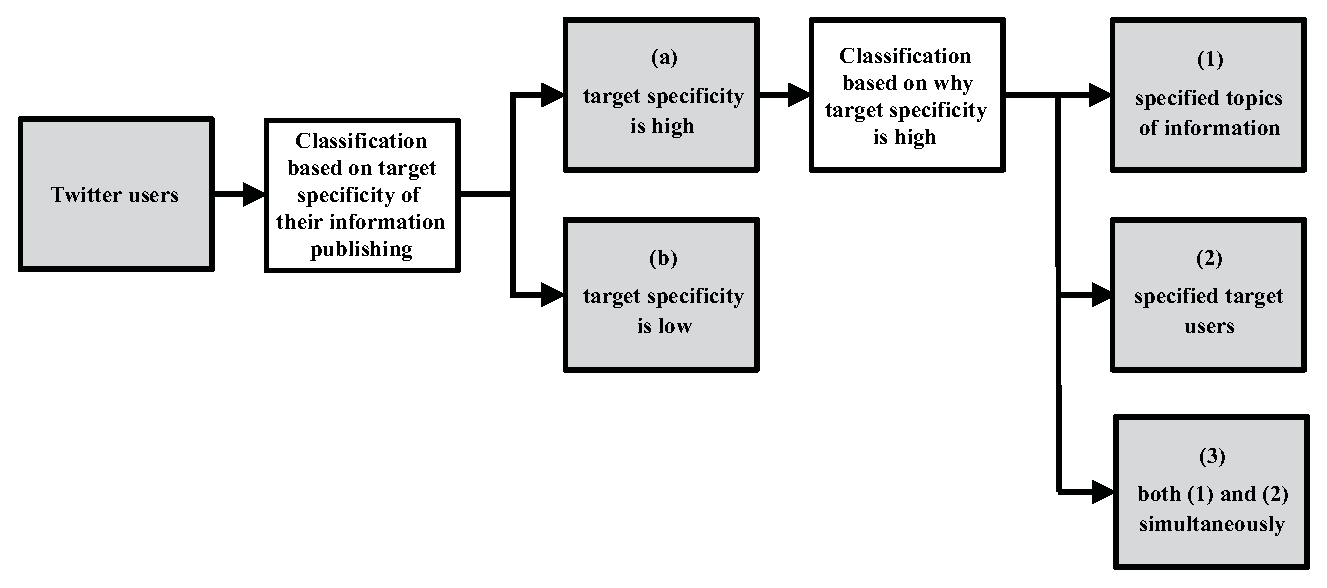
\includegraphics[width=14cm]{images/flow.eps}
 \caption{Overall flow of our methods}
\label{fig:Flow}
\end{center}
\end{figure}
}

In addition to this parameter: whether followers of a user are
consistent in a certain noticeable character or not, we consider
whether his/her follower set are covered with consistency subsets which
cover intermediately widely.  Here, \emph{a consistency subset} denotes
a subset which have consistency in a certain noticeable character.  As
show in Figure~\ref{fig:High Consistency} (b), in regard to followers of
a user, when half of them are consistent in the noticeable character $A$
and the others are consistent in the character noticeable $B$, it cannot
be said that they are consistent in one noticeable character, but
his/her follower set are covered with two consistency subsets which
cover intermediately widely.  In such a case, we consider that his/her
target specificity is high.

{\footnotesize
\begin{figure}[t]
\begin{center}
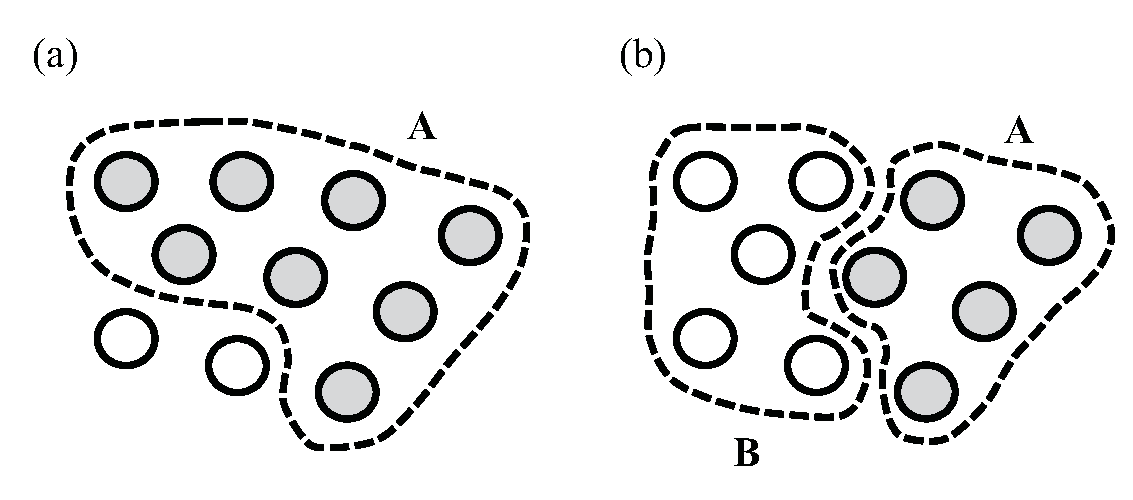
\includegraphics[width=14cm]{images/high_consistency.eps}
 \caption{Two examples of high target specificity}
\label{fig:High Consistency}
\end{center}
\end{figure}
}

These two parameters are summarized as follows.

\begin{description}
\item[(a)] The more consistent followers of a user are in a certain
           noticeable character, the higher his/her target specificity
           is.
\item[(b)] The more covered his/her follower set is with consistency
           subsets which cover intermediately widely, the higher his/her
           target specificity is.
\end{description}

The target specificity of a user is quite high when his/her followers
are consistent in one noticeable character, and it becomes lower as they
do not become consistent in any noticeable character.

Next, we explain the algorithm of computing a score of the target
specificity of a user $u$.

First, we collect all consistency subsets included in $u$'s follower set
$F_u$.  Then, in regard to each subset $S_{F_uc}$ which is consistent in
the character $c$ included in $F_u$, we compute
$\mathit{SubsetScore}(S_{F_uc})$ which denotes to what degree users in
$S_{F_uc}$ are consistent in $c$. We will propose two models which
compute $\mathit{SubsetScore}(S_{F_uc})$ in \ref{subsubsec:Scoring}.

Second, in descending order of $\mathit{SubsetScore}(S_{F_uc})$, we give
this score to each follower $f$ in $S_{F_uc}$ as
$\mathit{UserScore}_{\mathit{att}}(f)$, where $\mathit{att}$ means a
attribute measuring consistency, and we explain two attributes in
\ref{subsubsec:Attributes}. Here, we do not give a score to $f$ if
he/she already has a score. Then, we repeat this step over all
$\mathit{SubsetScore}(S_{F_uc})$.  In regard to users who are not given
a score after the above repeat, we set $0$ to them.  In other words, in
regard to each $f$ of $u$, we give
$\mathit{UserScore}_{\mathit{att}}(f)$ to the largest
$\mathit{SubsetScore}(S_{F_uc})$ of $S_{F_uc}$ in which $f$ is included
as follows:

\vspace{-1ex}
\[
 \mathit{UserScore}_{\mathit{att}}(f) = \max_{S_{F_uc} \in F_u}
 \{\mathit{SubsetScore}(S_{F_uc})|\;f \in S_{F_uc}\}.
\]
\vspace{-2ex}

Then, we take average of all $\mathit{UserScore_{\mathit{att}}(f)}$ for
$\mathit{SpecificityScore_{\mathit{att}}(u)}$, a score of the target
specificity of $u$, as follows:

\vspace{-1ex}
\[
 \mathit{SpecificityScore}_{\mathit{att}}(u) = \frac{1}{|F_u|}
 \sum_{f \in F_u} \mathit{UserScore}_{\mathit{att}}(f).
\]
\vspace{-2ex}

For example, suppose the case shown in Figure~\ref{fig:Algorithm}.
We assume that a follower set of a user $u$ have three consistency
subsets: $A$, $B$, and $C$, and $\mathit{SubsetScore}(A)$,
$\mathit{SubsetScore}(B)$, and $\mathit{SubsetScore}(C)$ are $3$, $2$,
and $1$ respectively.  In descending order of
$\mathit{SubsetScore}(S_{F_uc})$, i.e., in order of $A$, $B$, and $C$,
we give scores to each follower $f$ as
$\mathit{UserScore}_{\mathit{att}}(f)$ as shown in
Figure~\ref{fig:Algorithm}.  Finally, we compute average of
$\mathit{UserScore}_{\mathit{att}}(f)$ and take $2.6$ for
$\mathit{SpecificityScore_{\mathit{att}}(u)}$.

{\footnotesize
\begin{figure}[t]
\begin{center}
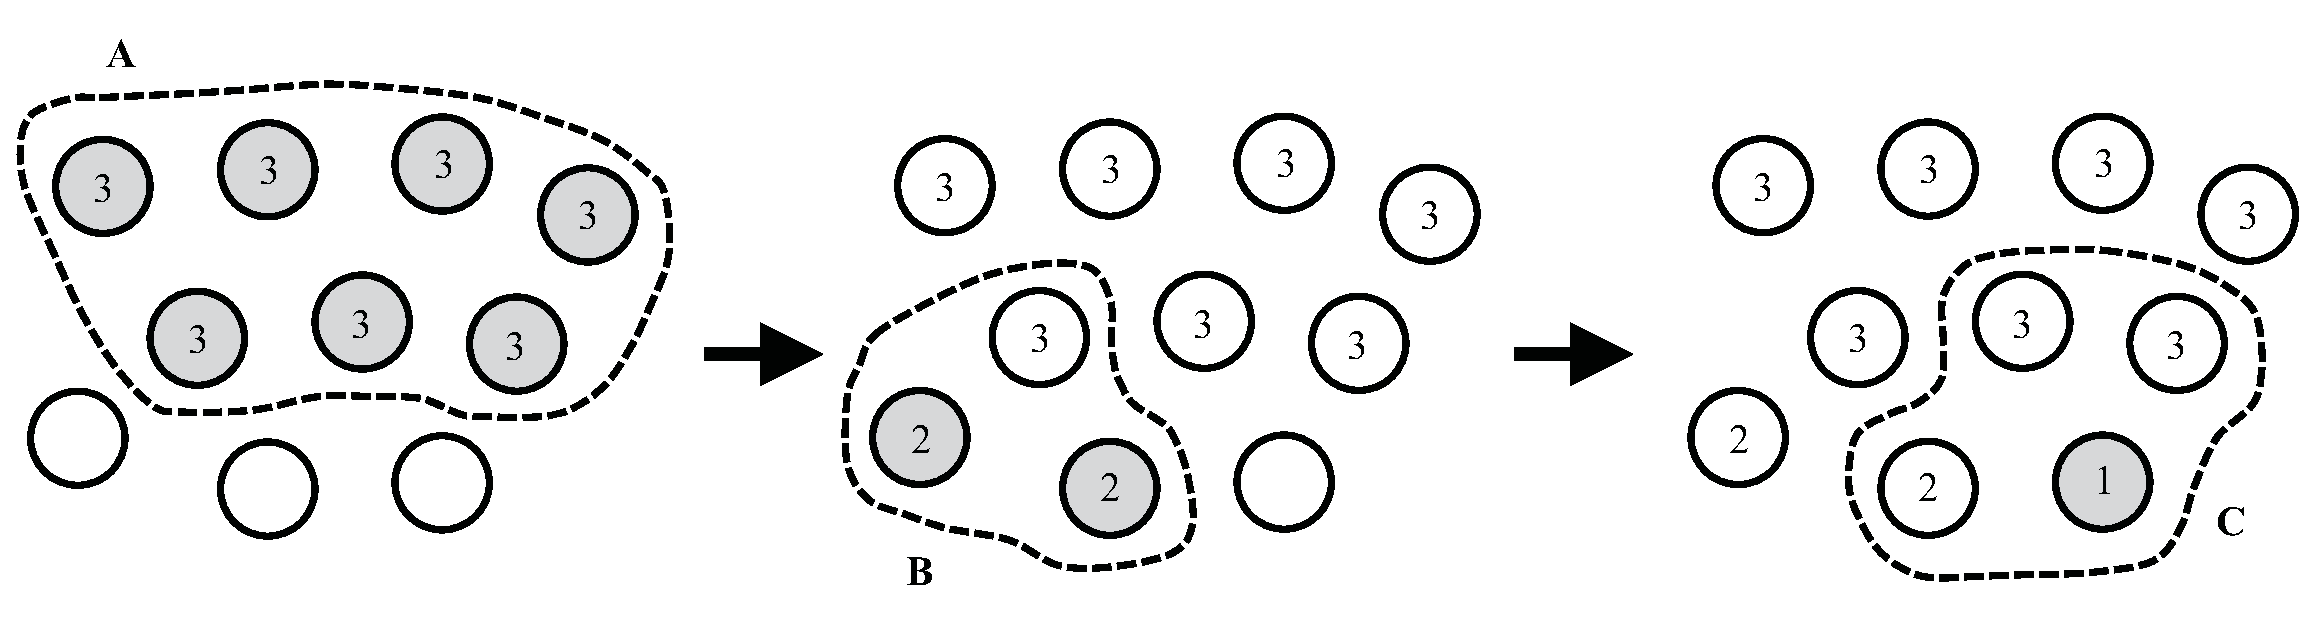
\includegraphics[width=14cm]{images/algorithm.eps}
 \caption{A case of the algorithm flow}
\label{fig:Algorithm}
\end{center}
\end{figure}
}

This is how we compute a score of the target specificity of $u$.  Below
is a summary of the algorithm:

\begin{description}
\item[1.]  we collect all consistency subsets including the follower set,
\item[2.]  we score each consistency subset based on to what degree users
           in it are consistent in a certain noticeable character
\item[3.]  in descending order of the above score, we repeatedly give it
           to each user in the subset, and
\item[4.]  we take average of scores for a score of the target
           specificity.
\end{description}

\subsubsection{Scoring Models of Consistency Subsets}
\label{subsubsec:Scoring}

In this subsubchapter, we explain a couple of models: (i) the
probabilistic model and (ii) the subtracting model which compute
$\mathit{SubsetScore(S_{F_uc})}$ mantioned in \ref{subsubsec:Algorithm}.
We explain these two models in the follow.

\begin{description}
\bf {\item[(i)] Probabilistic Model}
\end{description}

In this model, in regard to the consistency subset $S_{F_uc}$ which is
consistent in the character $c$ in the follower set $F_u$, we consider
that how low the probability that the user set of the same size as $F_u$
randomly sampled from the set of all Twitter users includes the subset
which is consistent in $c$ and whose size is $|S_{F_uc}|$ and over.
The lowness of the probability means that $S_{F_u}$ is inclining toward
a part of the set of all Twitter users, so it is able to be said that
$S_{F_uc}$ has consistency in a noticeable character if the probability
is low.  Thus, the lower the probability is, the higher score we give.
On the contrary, if the probability is
not so low,  the deviation between $S_{F_uc}$ and the user set randomly
sampled from all Twitter users may be small, and it is difficult to say
that $S_{F_uc}$ has consistency in a noticeable character.  Thus, we
give a low score in this case.

In addition to this parameter: how low the probability mentioned above
is, we consider that at what rate $S_{F_uc}$ covers with $F_u$.  The
more covered $F_u$ is with $S_{F_uc}$, the higher score we give.  Based
on these two parameters, we compute $\mathit{SubsetScore(S_{F_uc})}$.

These two parameters are summarized as follows.
\begin{itemize}
\item The lower the probability that the user set of the same size as $F_u$
randomly sampled from the set of all Twitter users includes the subset
which is consistent in the same character as the character of $S_{F_uc}$
and whose size is $|S_{F_uc}|$ and over, the higher score we give.
\item The more covered $F_u$ is with $S_{F_uc}$, the higher score we give.
\end{itemize}

Then, we define this model more formally.  First, we compute $P(u)$, the
probability that the user set of the size of $|F_u|$ randomly sampled
from the set of all Twitter users includes the subset which is
consistent in $c$ and whose size is $|S_{F_uc}|$, by the formula below:

\vspace{-1ex}
\[
 P(S_{F_uc}) = \int_{|S_{F_uc}|}^{n} \binom{n}{x} p^x (1-p)^{n - x}
 dx,\;\;\;\;\;n = |F_u|,\;\;\;\;\;p = \frac{|S_A|}{|A|}
\]
\vspace{-2ex}

\noindent{where $A$ is the set of all Twitter users, and $S_A$ is the subset which
is consistent in the character included in $A$.  The parameter $x$ in
the above formula is based on a binomial distribution.}

In addition, by adding the covering rate of $S_{F_uc}$ to $F_u$ to the
above parameter, we compute $\mathit{SubsetScore(S_{F_uc})}$.  However,
there is some possibility that $P(S_{F_uc})$ is excessively low because
$S_{F_uc}$ has a remarkable character, e.g., only a few users of all
users have the character, in spite of the size of $S_{F_uc}$ is very
small.  In this model, we expect that the consistency subset covers the
follower set at least intermediately widely.  So in such a case, we do
not give any scores to $S_{F_uc}$.  More specifically, we determine a
threshold $\gamma$ which cuts down the above case.

Then, we compute $\mathit{SubsetScore(S_{F_uc})}$ by the formula below:

%\vspace{-1ex}
%\[
% \mathit{SubsetScore}(S_{F_uc}) = \frac{|S_{F_uc}|}{|F_u|} \log (1 -
% P(S_{F_uc})).
%\]
%\vspace{-2ex}

\vspace{-1ex}
\[
  \displaystyle \mathit{SubsetScore}(S_{F_uc}) = \begin{cases}
    \displaystyle \frac{|S_{F_uc}|}{|F_u|} \log (1 - P(S_{F_uc})) &
    \mbox{if } \displaystyle \frac{|S_{F_uc}|}{|F_u|} > \gamma, \\
    \displaystyle \;\;\;\;\;0 & \mbox{otherwise.}
  \end{cases}
\]
\vspace{-2ex}

This is how we compute $\mathit{SubsetScore(S_{F_uc})}$ by using
probabilistic technique.

\begin{description}
 \bf {\item[(ii)] Subtracting Model}
\end{description}

In this model, in regard to the consistency subset $S_{F_uc}$, we
consider a covering rate of $S_{F_uc}$ to $F_u$ in comparison to a
covering rate of the subset which is consistent in the $c$ to the set of
all Twitter users.  We call the former \emph{a local rate} and the
latter \emph{a global rate}.  The fact that a local rate is high and a
global rate is low means $S_{F_uc}$ has consistency in a noticeable
character and is including toward a part of the set of all Twitter
users.  If a local rate is low or a global rate is high, it is difficult
to say that $S_{F_uc}$ has consistency in a noticeable character.  Based
on the above, we compute $\mathit{SubsetScore(S_{F_uc})}$ by the formula
below:

\vspace{-1ex}
\[
 \mathit{SubsetScore}(S_{F_uc}) = \max \{\frac{|S_{F_uc}|}{|F_u|} -
 \frac{|S_Ac|}{|A|}, 0\}.
\]
\vspace{-2ex}

In summary, we give a high score in the case of having the two features
simultaneously as follows:

\begin{itemize}
\item a covering rate of $S_{F_uc}$ to $F_u$ is high, and
\item a covering rate of the subset which is consistent in the same
      character as the character of $S_{F_uc}$ to the set of all Twitter
      users is low.
\end{itemize}

This is how we compute $\mathit{SubsetScore(S_{F_uc})}$by using
subtracting technique.

\subsubsection{Attributes for Extracting Consistency Subsets}
\label{subsubsec:Attributes}

In this subsubchapter, we explain a couple of attributes measuring
consistency: (i) common terms in profiles and location information, and
(ii) common followees.  By using these attributes, we extract
consistency subsets from the follower set of a user.  We explain these
two attributes in the follow.

\begin{description}
 \bf {\item[(i)] Common Terms in Profiles and Location Information}
\end{description}

As the first attribute measuring consistency, we consider common terms
included in profiles and local information of users in the follower set.

There is a high possibility that users belonging to the same community
or having the same interest have the same term in their profiles or
location information in common.  Thus, we extract such terms for
measuring consistency.  Here, we extract only noun phrases, which
characterize their profiles or location information strongly.

Based on the above, we define the method of extracting consistency
subsets more formally.  We compute the consistency subset $S_{F_ut}$
which is consistent in the term $t$ in $F_u$ by the formula below:

\vspace{-1ex}
\[
 S_{F_ut} =  \sum_{f \in F_u} \{f|\;t \in \mathit{Demography}(f) \}
\]
\vspace{-2ex}

\noindent{where $\mathit{Demography}(f)$ is the profile and location information
of $f$.  This is how we extract consistency subsets by using common
terms in profiles and location information.}


\begin{description}
 \bf {\item[(ii)] Common Followees}
\end{description}

As the second attribute measuring consistency, we consider common
followees of users in the consistency subset.

Users who are consistent in a certain noticeable character often have
the common tendency of the follow.  Users belonging to the same
community are dense on the social graph, so there is a high possibility
that they follow common users in the community.  And also, followers of
a user publishing technical information about programming is considered
to follow another user publishing useful information about programming
in common.  Thus, we focus on the tendency of the follow and extract
such followees for measuring consistency.

Based on the above, we define the method of extracting consistency
subsets more formally.  We compute the consistency subset $S_{F_ue}$
which is consistent in the followee $e$ in $F_u$ by the formula below:

\vspace{-1ex}
\[
 S_{F_ue} =  \sum_{f \in F_u} \{f|\;e \in E_f \}
\]
\vspace{-2ex}

\noindent{where $E_f$ is the followee set of $f$.  This is how we extract
consistency subsets by using common followees.}

\subsubsection{Final Classification Based on Target Specificity}
\label{subsubsec:Final Classification}

In this subsubchapter, we explain the method of computing the target
specificity of a Twitter user by using scores computed up to this
point.  In addition, based on the target specificity, we explain the
method of classifying users.

The $\mathit{SpecificityScore}_{{\mathit{att}}}(u)$ computed in
\ref{subsubsec:Algorithm} is higher in the cases that

\begin{itemize}
\item the more consistent followers of a user are in a noticeable
      character, or
\item the more covered his/her follower set are with consistency
      subsets which cover intermediately widely.
\end{itemize}

Then, we compute a score of the target specificity of $u$. We first
compute $\mathit{SpecificityScore}_{{\mathit{term}}}(u)$, which is using
common terms in profiles and location information as an attribute
measuring consistency mentioned \ref{subsubsec:Attributes} (i), and
$\mathit{SpecificityScore}_{{\mathit{followee}}}(u)$, which is using
common followees mentioned \ref{subsubsec:Attributes} (ii).  Then, we
take the larger one of these two scores for the target specificity of
$u$, because the larger one characterizes the target specificity more
strongly than the other.  More formally, we compute
$\mathit{TargetSpecificity}(u)$ by the formula below:

\vspace{-4ex}
\[
 \mathit{TargetSpecificity}(u) = \max \{
 \mathit{SpecificityScore}_{{\mathit{term}}}(u),
 \mathit{SpecificityScore}_{{\mathit{followee}}}(u)\}
\]
\vspace{-4ex}

Then, we determine a threshold $\delta$ which can classifies target
users and non target users accurately the most, and we classify them by
$\delta$.  More formally, we classify them as follows:

\vspace{-1ex}
\[
\begin{cases}
u\mbox{ is a } \mathit{target}\mbox{ }\mathit{user}, & \mbox{if}\
\mathit{TargetSpecificity}(u) > \delta \\
u\mbox{ is a }\mathit{non}\mbox{ }\mathit{target}\mbox{ }\mathit{user}, & \mbox{otherwise}.
\end{cases}
\]
\vspace{-2ex}

This is how we the target specificity of a Twitter user.

\subsection{Classifying Users of High Target Specificity}
\label{subsec:Classification Step2}

In this subsection, in regards to Twitter users classified into ``the
target specificity is high'' by the method mentioned in
\ref{subsec:Classification Step1}, we explain the method of determining
why their target specificities are high based on the result of our
analysis mentioned in \ref{subsec:The Causes}.

Here, we focus on the two causes of the high target specificity
mentioned in \ref{subsec:The Causes} as follows:
\begin{description}
 \item[(1)] because they publish information specified for certain
            topics, and
 \item[(2)] because they publish information to the users specified
            extensionally,
\end{description}

\noindent{and we determine whether a user we intend to classify
correlates with each cause mentioned above.}

We first determine various features of the user which potentially
correlate with each cause.  Then, based on these features, we construct
3-class classifiers which classify users into three categories: (1)
their target specificity is high because they publish information
specified for certain topics, (2) because they publish information to
the users specified extensionally, and (3) in the cause of both (1) and
(2).  By classifying users with the above classifiers, we determine why
their target specificities are high.

We adopted SVM and decision tree as a classifier.  Next, we explain what
features of users we used for the classification.  All the feature
values shown below were normalized to a value between $0$ and $1$.

\begin{description}
\bf {\item[(i)] numbers of followees and followers, and their ratio}
\end{description}

If the user publishes information to unspecified users, there is high
probability that a number of his/her followers is quite large or a
number of his/her followees is quite small.  So in such a case, a ratio
of a number of his/her followees to a number of his/her followers is
supposed to be very small.  Furthermore, if the user publishes
information to the closed users, i.e., his/her friends, his/her club
members, and so on, there is high probability that numbers of his/her
followers and followees are very close because the user is supposed to
have a reciprocal connection with them.  Thus, numbers of followees and
followers, and their ratio are useful for determining why their target
specificities are high.

\begin{description}
\bf {\item[(ii)] mutual follow ratio}
\end{description}

There is high probability that the user publishing information to the
closed users has a large mutual follow ratio, i.e., a number of users
with whom one follows one another is large, because the user is supposed
to have a reciprocal connection with them.  Therefore, a mutual follow
ratio is expected to be useful for determining why their target
specificities are high.

\begin{description}
\bf {\item[(iii)] frequency of replies by ``@''}
\end{description}

There is high probability that the user publishing information to the
closed users has a high frequency of replies by ``@'', i.e., the user
replies to his/her followers frequently. In regard to a mutual follow
ratio mentioned in (ii), there are some users publishing information to
unspecified users in spite of a large mutual follow ratio, but in regard
to a frequency of replies by ``@'', there is high probability that the
user publish information to the closed users.  This is because a high
frequency of replies by ``@'' demonstrates that the user is supposed to
have a reciprocal connection with them.  Therefore, a frequency of
replies by ``@'' is expected to be useful for determining why their
target specificities are high.

\begin{description}
\bf {\item[(iv)] partialness of topics in messages}
\end{description}

In regard to a user publishing information specified for certain topics,
topics in his/her messages are often partial.  Thus, we use the
partialness of topics in his/her messages as a feature for the
classification.

Then, we explain how to compute a partialness of topics in messages of
$u$.  We first collect up to 200 messages in order of newness.  Second,
we determine the topic of each message by using Latent Dirichlet
Allocation (LDA), which is a generative probabilistic model for
collections of discrete data such as text corpora.  Then, we compute
partialness of topics in messages $\mathit{partialness}(u)$ as follows:

\vspace{-3ex}
\[
 \mathit{partialness}(u) = - \sum_{t \in T_u} p_t \log p_t,\;\;\;\;\;
 p_t = \frac{|\{m|\;m \in M_u,\;\mathit{topic}(m) = t\}|}{|M_u|}
\]
\vspace{-3ex}

\noindent{where $M_u$ is a message set of $u$, $T_u$ is the topic set we
use for computing this feature, and $\mathit{topic}(m)$ is the topic of
a message $m$.  The partialness of topics $partialness(u)$ is the
entropy of $M_u$ on the topic.  This is how we compute a partialness of
topics in messages.}